\section{modelli biologici di crescita}
\index{modello!biologico}%

\subsection{modello di Malthus}
\index{modello!di Malthus}%
\index{Malthus!modello di}%
\index{esponenziale!modello di Malthus}%

Il più semplice modello di crescita di una popolazione è quello 
in cui si suppone che la popolazione abbia nutrimento e spazio sufficiente 
per una crescita indeterminata.
In questo modello la funzione $u(x)$ rappresenta la quantità di individui 
al tempo $x$ e si suppone che la velocità di crescita della popolazione $u'(x)$ 
sia proporzionale al numero di individui:
\[
  u'(x) = A u(x).  
\]
La soluzione di questa semplice equazione lineare (esercizio~\ref{ex:58230978})
è $u(x) = u_0\cdot  e^{A x}$ dove $u_0=u(0)$ è la popolazione al tempo 
iniziale $x=0$.
Significa che se $A>1$ la popolazione cresce indefinitamente tendendo 
a $+\infty$ per $x\to +\infty$ con velocità esponenziale.
Se $A<1$ invece la popolazione tende a zero (cioè si estingue)
sempre con velocità esponenziale.

\subsection{equazione logistica}
\index{equazione!logistica}%
\index{logistica!equazione differenziale}%
\index{crescita!logistica}%

Per rendere il modello di Malthus più realistico bisogna tenere conto 
del fatto che gli individui condividono uno spazio comune e che 
la presenza di molti individui nello stesso spazio diminuisce le risorse 
e quindi contribuisce in negativo alla crescita della popolazione. 
Supponiamo quindi che l'effetto negativo su una unità di popolazione 
sia proporzionale alla popolazione totale: $-Bu$ mentre l'aumento 
Malthusiano è sempre dato dal coefficiente $A$ per unità di popolazione. 
Si avrà quindi 
\[
  u'(x)  = (A-Bu(x))\cdot u(x)
\]
Questa è una equazione a variabili separabili. 
Le funzioni $u(x) = 0$ e $u(x) = \frac{A}{B}$ sono soluzioni 
stazionarie (ovvero costanti). 
La prima rappresenta una popolazione vuota, che quindi non potrà 
mai crescere. 
La soluzione $u=\frac{A}{B}$ rappresenta una popolazione 
in perfetto equilibrio.
Per semplificare le notazioni possiamo fare il cambio di variabile 
$v(x) = \frac{B}{A}\cdot u(x/A)$ che ci porta alla equazione 
equivalente $v'=(1-v)\cdot v$. 
Possiamo quindi supporre che sia $A=1$ e $B=1$ e ritornare 
alla variabile $u$:
\begin{equation}\label{eq:ode_logistica}
  u' = (1-u) u.  
\end{equation}

\newsavebox{\qrOdeLogistica}\sbox{\qrOdeLogistica}{%
\myqrshortdoclink{ode_logistica}{Le soluzioni dell'equazione logistica~\eqref{eq:ode_logistica}}}
\begin{figure}
  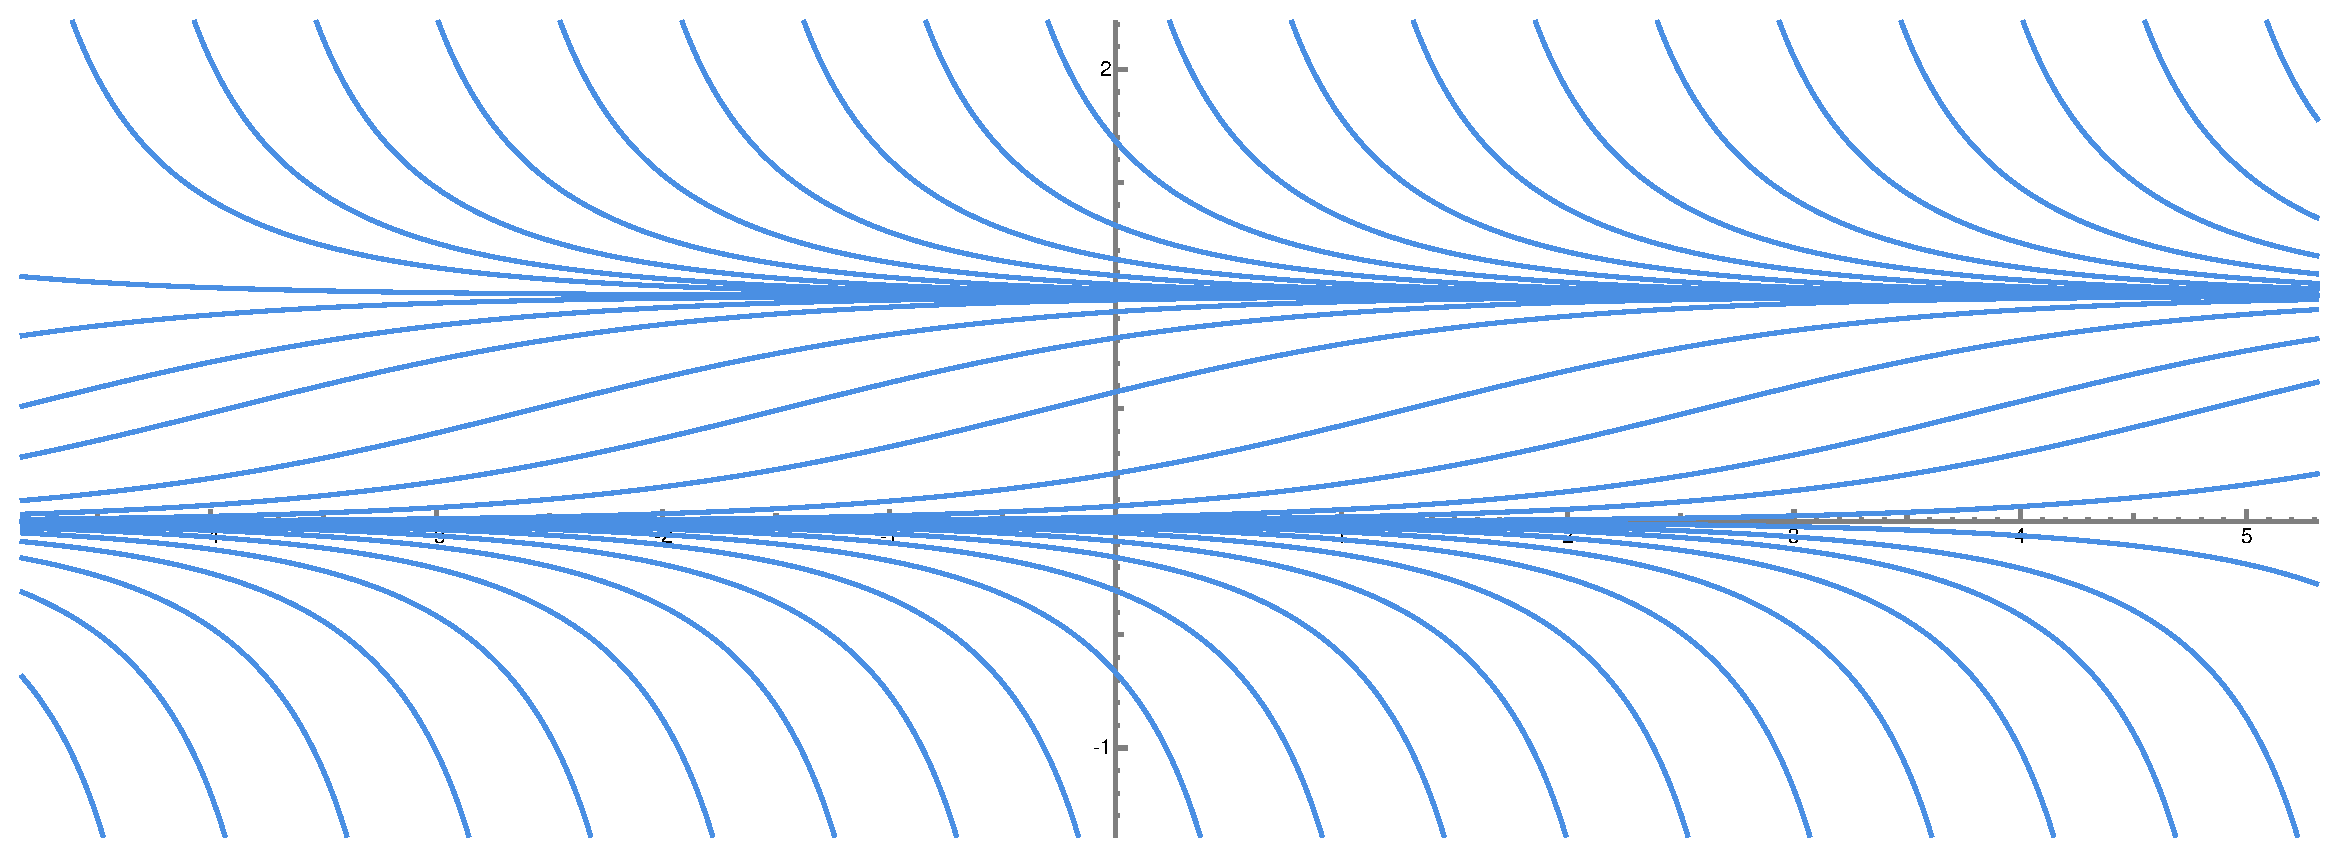
\includegraphics[width=\textwidth]{ode_logistica.pdf}
  \caption{
Le soluzioni dell'equazione logistica~\eqref{eq:ode_logistica}.
\ifwidemargin\\\\\fi%
\usebox{\qrOdeLogistica}}
\label{fig:ode_logistica}
\end{figure}

Avendo identificato le soluzioni stazionarie $u=0$ e $u=1$ possiamo separare le variabili
e integrare:
\[
 \int \frac{u'}{(1-u)u}\, dx = x - x_0.
\]
L'integrale si decompone con il metodo dei fratti semplici:
\[
  \int \frac{u'}{(1-u)u}\, dx
  = \int \frac{1}{(1-u)u}\, du 
  = \int \Enclose{\frac{1}{u} + \frac{1}{1-u}}\, du 
  = \ln \abs{u} - \ln\abs{1-u}
  = \ln \abs{\frac{u}{1-u}}.
\]
Dunque da 
\[
\abs{\frac{u}{1-u}} = e^{x-x_0}  
\]
si ottiene, con qualche passaggio algebrico,
\[
    u(x) = 1 - \frac{1}{1\pm e^{x-x_0}}.
\]
Il grafico di queste funzioni è rappresentato in figura~\ref{fig:ode_logistica}.
Nel capitolo~\ref{sec:studio_qualitativo_edo}
vedremo come risulta molto semplice ottenere l'andamento qualitativo dei grafici 
delle soluzioni di questa equazione senza doverne determinare esplicitamente 
le soluzioni.

\subsection{il modello di Volterra-Lotka}
\index{modello!di Volterra-Lotka}%
\index{Volterra!modello preda-predatore}%
\index{Lotka!modella preda-predatore}%
\index{preda/predatore}%

Il modello preda/predatore di Volterra-Lotka è il primo esempio 
di modello matematico applicato alla biologia.
\index{Volterra Vito}%
Il matematico italiano Vito Volterra si era interessato al problema 
di capire, tramite un modello matematico, il fenomeno apparentemente 
paradossale per cui il calo delle attività di pesca 
durante la prima guerra mondiale ha causato alla ripresa della pesca 
una diminuzione della 
quantità di pesce commestibile e un contemporaneo relativo aumento delle 
specie predatorie come gli squali.

Nel modello preda/predatore ideato da Volterra denotiamo con $u(x)$ 
la numerosità della popolazione di prede e con $v(x)$ la numerosità 
dei predatori al variare del tempo $x$.
Il modello è quindi rappresentato da un sistema di equazioni
non lineari del primo ordine:
\begin{equation}\label{eq:preda_predatore}
  \begin{cases}
    u' = A u - B u v \\
    v' = C u v - D v
  \end{cases}
\end{equation}
con $A,B,C,D$ costanti reali positive.
Il fattore di crescita delle prede è dettata da una legge di Malthus
$A u$ che rappresenta l'autosufficienza delle prede (si suppone 
abbiano sufficiente nutrimento per crescere indefinitamente).
L'addendo $-B u v$ rappresenta l'uccisione delle prede 
da parte dei predatori: è un termine proporzionale sia alla popolazione 
$u$ delle prede che alla popolazione $v$ dei predatori (come se ogni preda 
avesse un probabilità proporzionale a $v$ di incontrare un predatore).
Il termine $C u v$ rappresenta la corrispondente 
crescita dei predatori grazie al nutrimento dato dalle prede.
Viceversa i predatori non possono sostentarsi autonomamente e quindi 
il termine $-D v$ rappresenta l'estinguersi naturale dei predatori 
in assenza di nutrimento.

Alcune soluzioni del sistema~\eqref{eq:preda_predatore} possono essere 
trovate esplicitamente. 
Ad esempio se $v=0$ ci riconduciamo all'equazione di Malthus per $u$ 
e troviamo $u(x) = k e^{Ax}$: la preda cresce esponenzialmente in 
assenza di predatori.
Analogamente se $u=0$ si trova $v(x) = k e^{-Dx}$: i predatori 
si estinguono con velocità esponenziale in assenza di prede.


Possiamo inoltre trovare soluzioni stazionarie (cioè costanti) ponendo 
$u'=0$ e $v'=0$. Riscriviamo il sistema nella forma:
\begin{equation}\label{eq:preda_predatore_2}
  \begin{cases}
    u' = u \cdot (A - B v) \\
    v' = v \cdot (C u - D).
  \end{cases}
\end{equation}
e osserviamo quindi che per annullare contemporaneamente $u'$ e $v'$ 
si deve avere o $u=0$ e $v=0$ (soluzione in cui non ci sono né prede né predatori)
oppure si può avere $u=\frac D C$ e $v=\frac A B$ che è un punto di equilibrio
non banale tra le due specie.

Possiamo ottenere informazioni piuttosto precise 
se riusciamo ad identificare un integrale 
del sistema ovvero una funzione $H(u,v)$ che rimane costante sulle soluzioni: 
$\frac {d}{dx} H(u(x),v(x)) = 0$. 
Facendo il rapporto tra le due equazioni del sistema~\eqref{eq:preda_predatore_2}
si ottiene 
\[
  \frac{v'}{u'} 
  = \frac{v \cdot (C u - D)}{u \cdot (A - B v)}
\]
separando le variabili
\[
  \frac{A - B v}{v} v' = \frac{C u - D}{u} u'
\]
integrando in $dx$
\[
  \int \frac{A - B v}{v} v'\, dx  = \int \frac{C u - D}{u} u'  \, dx
\]
facendo i cambi di variabile $u=u(x)$, $v=v(x)$, $du = u'\, dx$, $dv=v'\, dx$
ed eseguendo le divisioni:
\[     
  \int \Enclose{\frac A v - B}\, dv = \int \Enclose{C  - \frac D u}\, du
\]
da cui, per una qualche costante $k$:
\[
  A \ln v - B v = C u - D\ln u + k.
\]
Significa che la funzione 
\[
  H(u,v) = B v + C u - A \ln v - D \ln u
\]
è costante lungo le curve $(u(x),v(x))$.
Dunque le traiettorie del sistema 
con $u>0$ e $v>0$ sono limitate, perché se 
$u$ oppure $v$ andassero all'infinito 
i termini $Bv-A\ln v$ o $Cu - D \ln u$ andrebbero 
anch'essi all'infinito e la funzione $H$ non 
potrebbe essere costante.

\newsavebox{\qrEdoVolterra}\sbox{\qrEdoVolterra}{%
  \myqrshortdoclink{edo_volterra}{Orbite del sistema preda/predatore~\ref{eq:preda_predatore}}}
\begin{figure}
  \begin{center}
    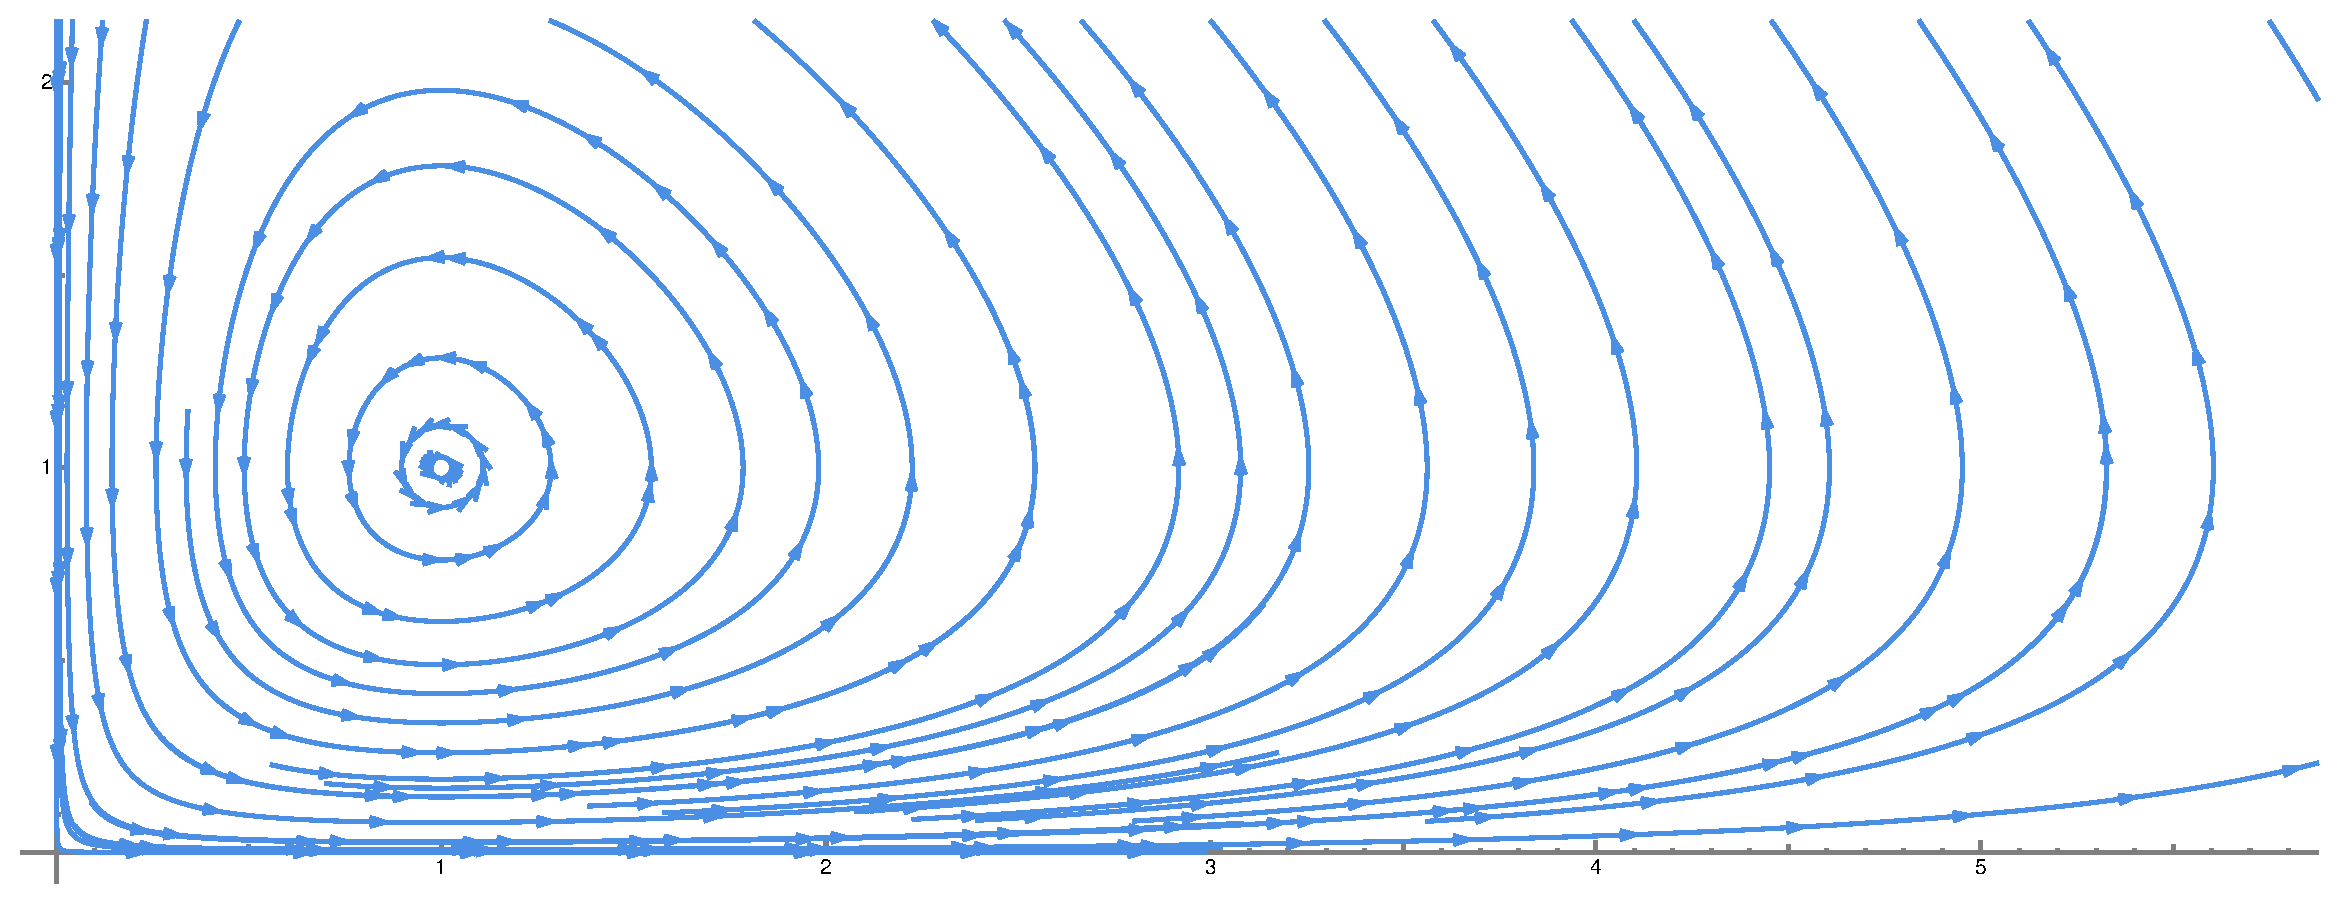
\includegraphics[width=\textwidth]{ode_volterra.pdf}
  \end{center}
  \caption{
  Le orbite del sistema preda/predatore~\eqref{eq:preda_predatore} 
  con la scelta dei parametri $A=B=C=D=1$.
  \ifwidemargin\\\\\fi%
  \usebox{\qrEdoVolterra}}
  \label{fig:ode_volterra}
\end{figure}

Consideriamo ora una soluzione $u(x),v(x)$ che al tempo $x_0$ 
si trova sul segmento $u=\frac DC$ e $v\in \openinterval{0}{\frac A B}$
(si faccia riferimento alla figura~\ref{fig:ode_volterra} dove abbiamo 
posto $\frac AB=1$ e $\frac DC=1$).
Siccome $v<\frac A B$ si ha $u'>0$ e quindi la curva si sposta verso destra.
Non appena $u>\frac DC$ si ha anche $v'>0$ e quindi la curva si sposta 
anche verso l'alto. Siccome $u$ non può tendere all'infinito 
prima o poi la soluzione deve raggiungere la retta $v=\frac AB$ 
dove la derivata di $u$ si annulla e la curva si sposta quindi 
in direzione verticale. Diventa quindi $v>\frac AB$ dove $u'<0$.
La coordinata $u$ dunque cala e siccome $v$ non può tendere all'infinito 
$u$ dovrà raggiungere il valore $\frac DC$ dove si ha $v'=0$.
Quindi si prosegue con $u<\frac DC$ dove $v'<0$.
Dunque ora sia $u$ che $v$ calano.
Devono però rimanere positivi sia perché la funzione $H$ tende all'infinito 
anche quando $u\to 0$ o $v\to 0$ sia perché gli assi $u=0$ e $v=0$ 
sono orbite delle soluzioni esplicite che abbiamo trovato inizialmente 
e per l'unicità delle soluzioni non è possibile che orbite diverse 
si incontrino in un punto.
Dunque ad un certo punto si avrà di nuovo $v= \frac AB$ e $u\in \openinterval{0}{\frac DC}$
e poi si avrà $v<\frac AB$ con $u'>0$ e $v'<0$.
La nostra curva dovrà quindi di nuovo raggiungere in un istante $x_1>x_0$ 
il segmento da cui 
eravamo partiti: $u=\frac DC$ e $v\in \openinterval{0}{\frac AB}$.
In tutto questo percorso $H$ è rimasta costante dunque si avrà 
$H(u(x_1),v(x_1))=H(u(x_2),v(x_2))$. 
Ma $u(x_1)=u(x_2) = \frac DC$ e posto $f(v) = H(D/C,v)$ si osserva che 
\begin{align*}
   f(v) = B v + D - A \ln v - D \ln \frac DC.
\end{align*}
studiando il segno della derivata $f'(v)=B-\frac{A}{v}$ si osserva che per $v<\frac AB$ 
la derivata è strettamente negativa dunque la funzione $f$ è strettamente 
decrescente nell'intervallo $v\in(0,D/C)$ dunque iniettiva.
Essendo $f(v(x_1)) = f(v(x_2))$ deduciamo quindi che $v(x_1)=v(x_2)$.
Significa che la curva si richiude e le soluzioni sono dunque 
periodiche di periodo $T=x_2-x_1$. 

Preso un qualunque punto del quadrante $u>0$, $v>0$ (escluso il punto
critico) la soluzione che parte
da quel punto seguirà un percorso che, in base alle considerazioni che abbiamo già 
fatto, è costretto prima o poi ad attraversare il segmento che abbiamo 
preso in considerazione e quindi è, in effetti, una di quelle che 
abbiamo già studiato.

Questo studio qualitativo descrive l'andamento delle soluzioni 
del sistema~\ref{eq:preda_predatore}: si cerchi di interpretare 
il significato biologico di quanto abbiamo dedotto. Metodi numerici 
(come quelli utilizzati per ottenere la figura~\ref{fig:ode_volterra})
ci permettono di ottenere informazioni quantitative con la precisione 
desiderata.

Possiamo ora anche rispondere alla domanda iniziale rivolta a Vito Volterra 
e cioè spiegare cosa succede in presenza dell'attività umana di pesca.
Il sistema studiato finora è quello che descrive l'andamento in assenza 
dell'attività di pesca (cioè quanto veniva osservato dai naturalisti alla fine della 
prima guerra mondiale). 
In presenza di pesca intensiva dobbiamo supporre che la quantità di pesce 
pescato è proporzionale, per ogni specie, alla numerosità della specie stessa.
Dunque dobbiamo sottrarre un termine $Eu$ dalla prima equazione e un termine 
corrispondente $Ev$ dalla seconda:
\begin{equation}
  \begin{cases}
    u' = A u - B u v - Eu = (A-E) u - B uv\\
    v' = C u v - D v - Ev = C uv - (D+E) v.
  \end{cases}
\end{equation}
Si osserva quindi che il sistema rimane dello stesso tipo solo che 
il coefficiente $A$ è diminuito diventando $A-E$ mentre il coefficiente 
$D$ è aumentato diventando $D+E$.
Dunque il punto di equilibrio $u=\frac DC$, $v=\frac AB$ si è spostato 
verso destra e verso il basso in quanto $D$ è aumentato e $A$ è diminuito.
Questo significa che in media l'attività di pesca favorisce un aumento 
delle prede e una diminuzione dei predatori. 
Viceversa la diminuzione dell'attività di pesca fa diminuire la quantità
di prede e aumentare quella dei predatori.

